\documentclass{article}
\usepackage{amsmath}
\usepackage{tcolorbox}
\usepackage{graphicx,wrapfig,lipsum}
\usepackage{epstopdf}
\begin{document}


\includegraphics[scale=0.7]{puzzles.eps}

\begin{tcolorbox}
%------------------------------------------
\begin{wrapfigure}{r}{5.5cm}
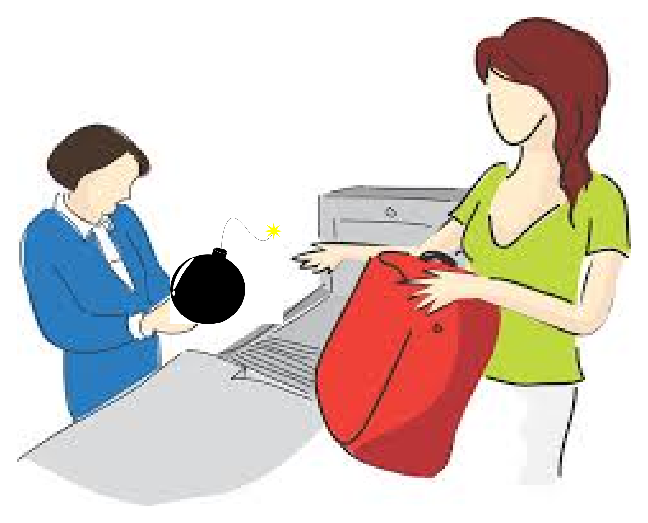
\includegraphics[width=5.5cm]{bmb.eps}
\end{wrapfigure} 
%------------------------------------------
A mathematician was flying from England to Canada. While boarding onto the flight, she was arrested for hiding a bomb in her bag. When enquired, she said, ``I did it in order to reduce the probability of the flight being blasted by a bomb". Observing the confused faces, she further explained that one in $1000$ persons might carry a bomb in the flight. Hence, the probability of a person carrying a bomb in the flight = $\frac{1}{1000}$, which is not very less. Hence, it was difficult for her to have her peace of mind while flying. Even now, the reason for her carrying a bomb was not clear. She further explained; the probability of two people carrying a bomb in the flight = $\frac{1}{1000} \times \frac{1}{1000}\ = \frac{1}{1000000}$, which is very very less. Confused authorities asked her, ``So what? How does that justify you carrying a bomb?". She said; if she carries a bomb, then since the probability of two people carrying bombs is very less; hence, the probability of another bomb on the flight reduces drastically. 

\textbf{To ponder over:} What went wrong about the mathematician's reasoning?

\end{tcolorbox}

\begin{tcolorbox}
%------------------------------------------
\begin{wrapfigure}{r}{4cm}
\begin{flushleft}
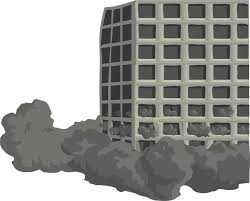
\includegraphics[width=3cm]{building.jpeg}
\end{flushleft}
\end{wrapfigure} 
%------------------------------------------
Imagine a very old building standing intact from millions of years. Let $P(today)$ = The probability that this building will fall today and $P(tomorrow)$ = The probability that this building will fall tomorrow. 

\textbf{To ponder over}: Whether $P(today)<P(tomorrow)$, or $P(today)>P(tomorrow)$ or $P(today)=P(tomorrow)$ ?

\end{tcolorbox}

\begin{tcolorbox}
%------------------------------------------
\begin{wrapfigure}{r}{4cm}
\begin{flushleft}
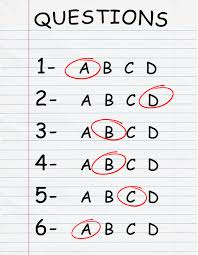
\includegraphics[width=3cm]{omr.jpeg}
\end{flushleft}
\end{wrapfigure} 
%------------------------------------------
Consider a multiple choice exam conducted countrywide. There are two students- $A$ and $B$. $A$ and $B$ both have scored equal marks. But while $A$ has attempted the questions geuinely; $B$ has randomly answered the questions and became lucky enough to score equal to $A$. 

\textbf{To ponder over:} By looking at their OMR\footnote{Optical Mark Reading- One where we darken the bubbles corresponding to the correct answer- A/B/C/D.} sheets (without knowing which sheet belongs to whom), can one predict their corresponding sheets?


\end{tcolorbox}

\end{document}